% Provenance (never printed): cycle 4 SVT, "La planete Terre, l'environnement
% et l'action humaine": climate, its past variations and the present change,
% read from data; see sources/book1/PROVENANCE.md. Book 1, grade 9, chapter 1.
% Vocabulary guard: owns climate change (first look; Book 2 g12 re-uses it),
% global warming, temperature anomaly. The greenhouse effect and greenhouse
% gases belong to the chemistry series (grade 8): recalled in prose, never
% defined. Infrared is physics (g10): named in prose only. "Glacial period"
% and "interglacial" belong to Book 2 g12: here "the ice ages and the warmer
% times between them". Physical science only, in the IPCC's calibrated words;
% no policy.
\chapter{Le climat de la Terre, hier et aujourd'hui}\label{ch:g9:climate-past-and-present}

Si la Terre n'avait pas d'air autour d'elle, tout en réfléchissant la même
part de la lumière du Soleil qu'aujourd'hui, sa surface se stabiliserait à
une température moyenne d'environ \qty{-19}{\degreeCelsius}~: des \omterm{def:g2:water-on-earth:ocean}{mers}
gelées, des terres gelées, partout. Sa moyenne réelle est d'environ
\qty{15}{\degreeCelsius}. La différence, quelque \qty{34}{\degreeCelsius},
vient de quelques gaz de l'air, présents en quantités infimes, qui
empêchent une partie de la chaleur de la Terre de s'échapper vers
l'espace. Ce chapitre parle de ces gaz, du \omterm{def:g5:weather-and-climate:climate}{climat} passé de la Terre, et
de la manière dont il change aujourd'hui, et pourquoi.
% ledger: earth:Tbb, earth:Tsurf (figdata/grade-9/climate_records.py: -19.1 and 14.9 degC, gap 34)

\begin{recall}
Le \omterm{def:g5:weather-and-climate:climate}{climat} d'un lieu est le temps qu'il y fait habituellement, en moyenne
sur 30 ans (\cref{ch:g5:weather-and-climate}). La couche la plus basse de
l'atmosphère, celle où se fait le temps, est la \omterm{def:g8:the-atmosphere:layers}{troposphère}
(\cref{ch:g8:the-atmosphere}). Les \omterm{def:g8:ice-on-earth:ice-age}{glaciations}, avec leurs \omterm{def:g8:ice-on-earth:ice-sheet}{calottes
glaciaires} étendues bien au-delà des \omterm{def:g3:continents-and-oceans:poles}{pôles}, sont venues et reparties~; la
\omterm{def:g8:ice-on-earth:sea-ice}{banquise} arctique a diminué depuis 1979 (\cref{ch:g8:ice-on-earth}). En
chimie, on apprend que le dioxyde de carbone, le méthane et la vapeur
d'eau sont des \emph{gaz à effet de serre}~: ils laissent passer la
lumière du Soleil mais absorbent la lumière infrarouge invisible émise par
le sol chaud, c'est l'\emph{effet de serre}~; brûler du charbon, du
pétrole et du gaz libère du dioxyde de carbone.
\end{recall}

\section{L'effet de serre et la température de la Terre}

La lumière du Soleil traverse l'atmosphère et réchauffe le sol et les
\omterm{def:g2:water-on-earth:ocean}{océans}. Comme tout corps chaud, la surface chauffée émet à son tour de
l'énergie, sous forme de lumière infrarouge que l'œil ne peut pas voir. Si
toute cette énergie s'échappait vers l'espace, la Terre serait le monde
gelé du premier paragraphe. Mais les gaz à effet de serre de l'air
absorbent une grande partie de cette lumière infrarouge et en renvoient
une part vers le bas~: la surface reçoit de l'énergie à la fois du Soleil
et de l'air au-dessus d'elle, et se stabilise à une température plus
élevée.

\begin{omfigure}
\begin{tikzpicture}[font=\footnotesize, >={Stealth[length=2.4mm]}]
  % ground and atmosphere
  \fill[omLithAlluv] (0,0) rectangle (12,0.5);
  \fill[omSea!45] (0,0.5) rectangle (12,3.4);
  \node[anchor=north east, align=right] at (11.85,3.35) {atmosphère avec des\\ gaz à effet de serre};
  \node[anchor=south east] at (11.9,0.05) {sol et océans};
  \node[anchor=south west] at (0.15,3.5) {espace};
  % Sun
  \fill[omWxSun] (1.3,5.0) circle (0.45);
  \node at (1.3,4.3) {Soleil};
  % sunlight in
  \draw[->, omWxSun!80!black, line width=2.2pt] (1.7,4.6) -- (2.7,0.55)
    node[pos=0.25, right=2pt, align=left, black] {la lumière du Soleil entre\\ et réchauffe la surface};
  % infrared out and back
  \draw[->, omWarm, line width=1.6pt, decorate, decoration={snake, amplitude=1mm, segment length=4mm, post length=3mm}]
    (6.0,0.55) -- (6.6,2.6);
  \draw[->, omWarm, line width=1.6pt, decorate, decoration={snake, amplitude=1mm, segment length=4mm, post length=3mm}]
    (6.6,2.7) -- (7.4,5.0) node[right, align=left, black] {une partie s'échappe\\ vers l'espace};
  \draw[->, omWarm, line width=1.6pt, decorate, decoration={snake, amplitude=1mm, segment length=4mm, post length=3mm}]
    (6.8,2.75) -- (8.6,0.55);
  \node[align=left, anchor=west] at (8.8,1.55) {une partie est\\ absorbée par les gaz\\ et renvoyée\\ vers le bas};
  \node[align=right, anchor=east] at (5.9,1.3) {la surface chaude\\ émet de l'infrarouge};
\end{tikzpicture}

{\small L'effet de serre, en simplifiant (un croquis). Sans lui, la surface
de la Terre aurait une température moyenne d'environ
\qty{-19}{\degreeCelsius}~; avec lui, d'environ \qty{15}{\degreeCelsius}.}
% ledger: earth:Tbb, earth:Tsurf
\label{fig:g9:climate-past-and-present:greenhouse}
\end{omfigure}

L'effet de serre est naturel et nécessaire~: sans lui, il n'y aurait pas
d'eau liquide à la surface. La question de ce chapitre est autre~: que
devient la température de la Terre quand la quantité de gaz à effet de
serre dans l'air change~?

\section{Les climats du passé}

Pour lire le \omterm{def:g5:weather-and-climate:climate}{climat} d'un passé lointain, les scientifiques forent les
\omterm{def:g8:ice-on-earth:ice-sheet}{calottes glaciaires}. Chaque année, de la \omterm{def:g4:clouds-rain-snow:precipitation}{neige} tombe sur l'Antarctique et
le Groenland, et la \omterm{def:g4:clouds-rain-snow:precipitation}{neige} d'été est un peu différente de la \omterm{def:g4:clouds-rain-snow:precipitation}{neige}
d'hiver. Enfouies et tassées en glace, les couches annuelles restent, les
unes au-dessus des autres, comme les pages d'un livre. Plus la glace est
profonde, plus elle est ancienne.
% ledger: eo:ice-core

\begin{omfigure}
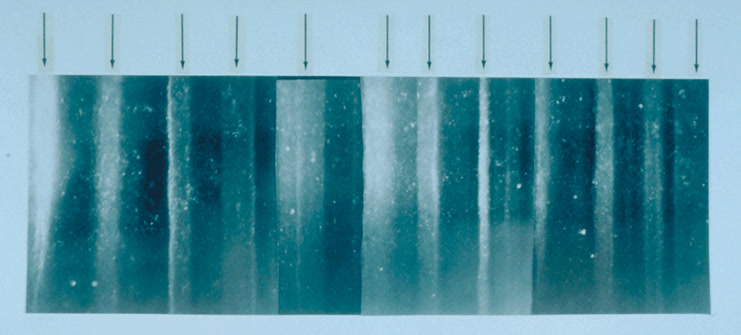
\includegraphics[width=0.78\linewidth]{images/book1/g9-gisp2-layers.jpg}

{\small Un tronçon de carotte de glace long de \qty{19}{cm}, prélevé à
\qty{1855}{m} de profondeur dans la calotte du Groenland et éclairé par en
dessous. Les flèches désignent les couches d'été, plus claires, entre des
couches d'hiver plus sombres~: onze années de \omterm{def:g4:clouds-rain-snow:precipitation}{neige}. NOAA Paleoclimatology
(domaine public, via Wikimedia Commons).}
% ledger: commons:gisp2-layers
\label{fig:g9:climate-past-and-present:ice-core}
\end{omfigure}

Une carotte de glace garde deux archives du passé. La \omterm{def:g4:clouds-rain-snow:precipitation}{neige} elle-même
indique quel froid il faisait quand elle est tombée~: plus l'air était
froid, plus la part des formes lourdes de l'hydrogène et de l'oxygène dans
la \omterm{def:g4:clouds-rain-snow:precipitation}{neige} était faible. Et quand la \omterm{def:g4:clouds-rain-snow:precipitation}{neige} se tasse en glace, les espaces
entre les grains se ferment et emprisonnent de minuscules bulles de l'air
de l'époque. Les scientifiques libèrent cet air ancien au laboratoire et
mesurent son dioxyde de carbone.
% ledger: eo:ice-core

\begin{omfigure}
\begin{tikzpicture}
\begin{axis}[name=temp, omrecord, omage, width=13cm, height=3.9cm, xmin=0, xmax=800,
  xtick={0,100,...,800}, xticklabels={}, ylabel={variation de\\ température ($^\circ$C)},
  ylabel style={align=center}, ymin=-11, ymax=5, ytick={-10,-5,0,5}]
  \addplot[omWarm, line width=0.7pt] table[x=age_kyr, y=temp_C] {figdata/out/grade-9-climate_records-edc.dat};
\end{axis}
\begin{axis}[at={(temp.south west)}, anchor=north west, yshift=-0.3cm, omrecord, omage,
  width=13cm, height=3.9cm, xmin=0, xmax=800, xtick={0,100,...,800},
  xlabel={milliers d'années avant aujourd'hui}, ylabel={dioxyde de\\ carbone (ppm)},
  ylabel style={align=center}, ymin=160, ymax=320, ytick={180,220,260,300}]
  \addplot[black, line width=0.7pt] table[x=age_kyr, y=co2_ppm] {figdata/out/grade-9-climate_records-icecore.dat};
\end{axis}
\end{tikzpicture}

{\small Huit cent mille ans lus dans la glace de l'Antarctique. En haut~:
la variation de la température de l'air au Dôme~C, par rapport à la
moyenne des mille dernières années (carotte de glace EPICA Dôme~C,
J.~Jouzel et al., 2007). En bas~: le dioxyde de carbone de l'air piégé
dans la glace, en parties par million (B.~Bereiter et al., 2015). Les deux
sont moyennés par pas de \num{2000} ans~; le temps va de la gauche (le
plus ancien) vers la droite (aujourd'hui).}
% ledger: data:edc-jouzel, data:co2-bereiter (figdata/grade-9/climate_records.py)
\label{fig:g9:climate-past-and-present:icecore}
\end{omfigure}

Les deux courbes racontent la même histoire. Encore et encore, de longues
périodes froides, les \omterm{def:g8:ice-on-earth:ice-age}{glaciations}, ont cédé la place à des périodes
chaudes plus courtes, puis le froid est revenu. Au plus froid, l'air
au-dessus de l'Antarctique était d'environ \qty{9}{\degreeCelsius} plus
froid que pendant les mille dernières années~; aux périodes les plus
chaudes, il était plus chaud de quelques degrés. Et le dioxyde de carbone
montait et descendait avec la température, entre environ \qty{175}{ppm}
pendant les périodes froides et environ \qty{300}{ppm} pendant les
périodes chaudes. Nous vivons dans l'une de ces périodes chaudes, qui a
commencé à la fin de la dernière \omterm{def:g8:ice-on-earth:ice-age}{glaciation}.
% ledger: data:edc-jouzel, data:co2-bereiter (figdata/grade-9/climate_records.py: edc min -9.7, max +3.6; CO2 174 to 299 ppm)

\begin{method}[Lire deux archives côte à côte]
\begin{enumerate}
  \item Vérifie que les deux archives ont le même axe du temps, et dans
        quel sens le temps s'écoule.
  \item Choisis une date sur l'axe du temps et lis chaque archive à cette
        date.
  \item Cherche les pics et les creux~: arrivent-ils aux mêmes moments
        dans les deux archives~?
  \item Dis ce qui varie ensemble, sans décider encore quel changement a
        causé l'autre.
\end{enumerate}
\end{method}

\begin{example}[La dernière glaciation dans la carotte de glace]
À \num{20000} ans avant aujourd'hui (le 20 sur l'axe du temps), la courbe
des températures est à environ \qty{-9}{\degreeCelsius} et le dioxyde de
carbone à environ \qty{190}{ppm}. Pendant les mille dernières années, la
courbe des températures est proche de 0 et le dioxyde de carbone proche de
\qty{280}{ppm}. Ainsi, au plus froid de la dernière \omterm{def:g8:ice-on-earth:ice-age}{glaciation}, l'air
au-dessus de l'Antarctique était plus froid d'environ
\qty{9}{\degreeCelsius}, et il contenait environ
$280 - 190 = \qty{90}{ppm}$ de dioxyde de carbone en moins, un tiers de
moins.
\end{example}
% ledger: data:edc-jouzel, data:co2-bereiter (figdata/grade-9/climate_records.py: 19-21 kyr bins -9.4, 190 ppm; 1 kyr bin 278)

Plus loin encore dans le passé, la Terre a connu des \omterm{def:g5:weather-and-climate:climate}{climats} bien plus
chauds que tous ceux des 800\,000 dernières années. Les évaluations
scientifiques estiment que la dernière fois que la surface de la Terre
est restée \qty{2.5}{\degreeCelsius} ou plus au-dessus de son niveau de la
fin du \textsc{xix}\textsuperscript{e}~siècle remonte à plus de trois
millions d'années.
% ledger: ipcc:3myr

\section{Les mesures d'aujourd'hui}

Depuis la fin du \textsc{xix}\textsuperscript{e}~siècle, la température
est mesurée chaque jour dans des milliers de stations \omterm{def:g1:watching-the-weather:weather}{météorologiques}, sur
terre et en \omterm{def:g2:water-on-earth:ocean}{mer}, avec des thermomètres placés à l'ombre. Pour suivre la
planète entière, les scientifiques ne font pas la moyenne des températures
elles-mêmes, qui dépendent de l'endroit où se trouve chaque station, mais
de l'écart de chacune à sa propre valeur habituelle.
% ledger: giss:method

\begin{definition}[Anomalie de température]\label{def:g9:climate-past-and-present:anomaly}
Une \emph{anomalie de température}\index{anomalie de temperature@anomalie de température} est la différence
entre une température et sa moyenne sur une période de référence choisie.
Elle est positive quand il fait plus chaud que cette moyenne, négative
quand il fait plus froid.
\end{definition}

\begin{omfigure}
\begin{minipage}[c]{0.44\linewidth}\centering
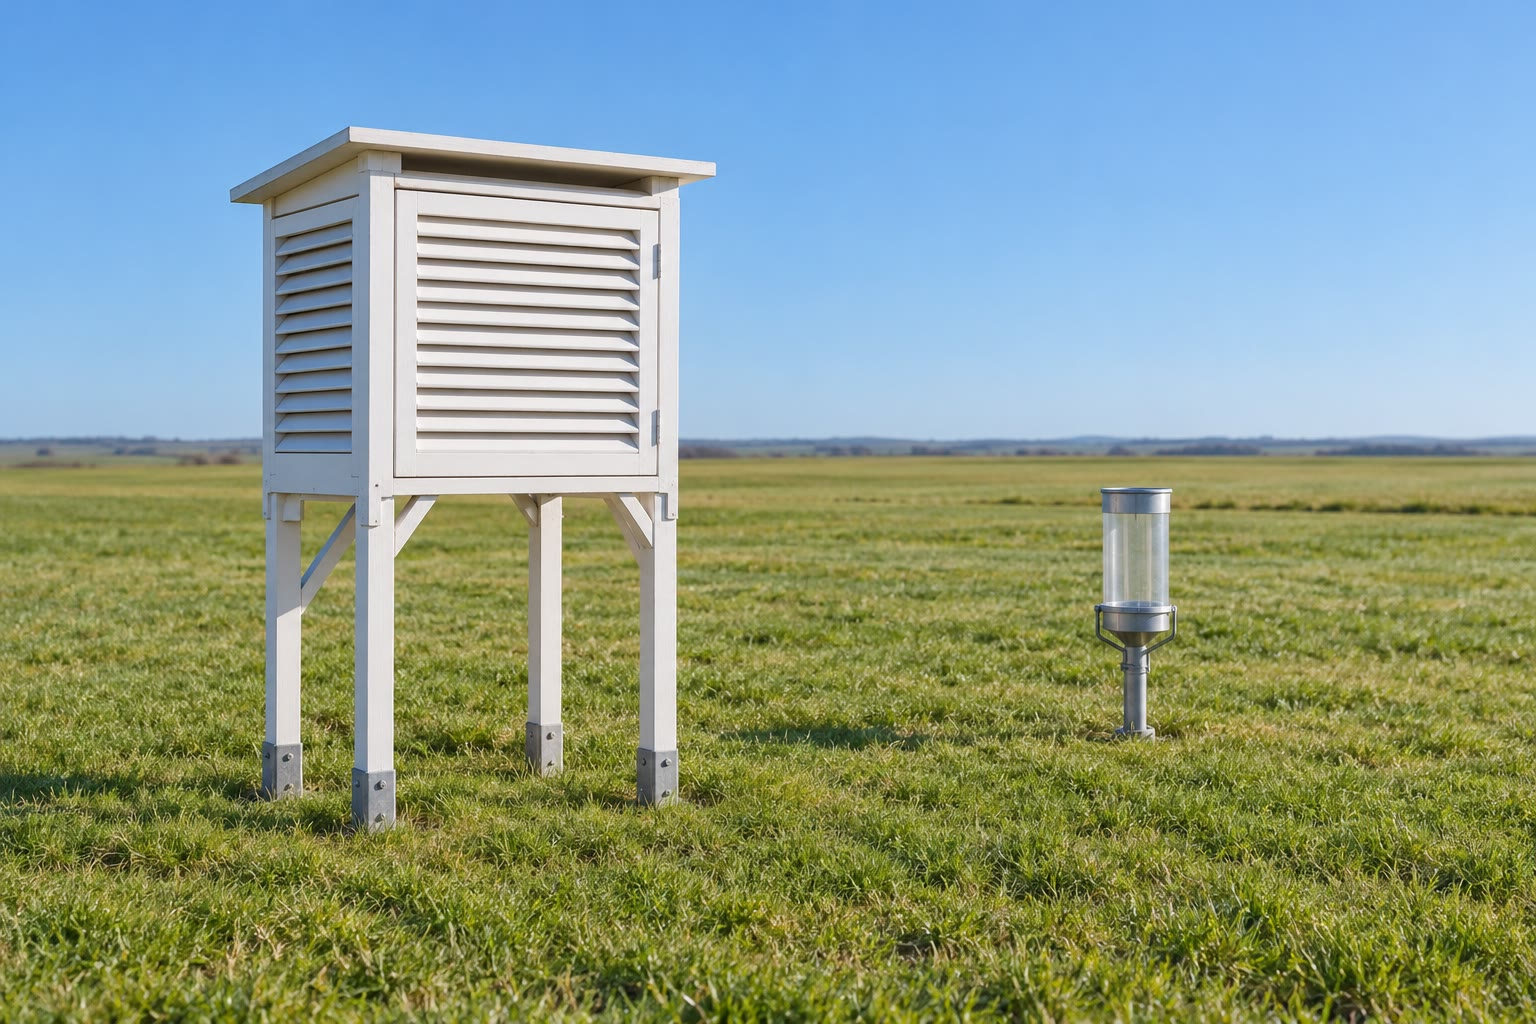
\includegraphics[width=\linewidth]{images/book1/ai/g9-weather-screen.jpg}
\end{minipage}\hfill
\begin{minipage}[c]{0.52\linewidth}\raggedright
{\small Une station \omterm{def:g1:watching-the-weather:weather}{météorologique}~: l'abri blanc sur pieds, aux parois
à persiennes, garde les thermomètres à l'ombre tout en laissant l'air
circuler~; à droite, un \omterm{def:g4:clouds-rain-snow:rain-gauge}{pluviomètre} (illustration générée par IA d'une
scène générique).}
\end{minipage}
\label{fig:g9:climate-past-and-present:screen}
\end{omfigure}

La série des températures mondiales de la NASA, par exemple, donne
l'anomalie de chaque année par rapport à la moyenne de 1951--1980, à partir
de stations sur terre et de mesures de la surface de la \omterm{def:g2:water-on-earth:ocean}{mer}. En moyenne
décennie par décennie, elle montre une nette hausse.
% ledger: giss:method, data:gistemp

\begin{omfigure}
\begin{tikzpicture}
\begin{axis}[omrecord, ybar, width=13cm, height=5.6cm, bar width=9pt,
  ymin=-0.45, ymax=1.2, ytick={-0.4,0,0.4,0.8,1.2},
  xtick=data, xticklabels={années 1880, années 1890, années 1900, années 1910, années 1920, années 1930, années 1940, années 1950, années 1960, années 1970, années 1980, années 1990, années 2000, années 2010, 2020--2025},
  x tick label style={rotate=60, anchor=east, font=\scriptsize},
  ylabel={anomalie de température ($^\circ$C)}, xmajorgrids=false]
  \addplot[fill=omWarm!70, draw=black!50] table[x expr=\coordindex, y=mean_C]
    {figdata/out/grade-9-climate_records-decades.dat};
\end{axis}
\end{tikzpicture}

{\small La température de surface du \omterm{def:g3:continents-and-oceans:globe}{globe}, décennie par décennie depuis
les années 1880, sous forme d'anomalie par rapport à la moyenne de
1951--1980~; la dernière barre couvre les six années 2020--2025.
Données~: NASA GISTEMP version~4.}
% ledger: data:gistemp (figdata/grade-9/climate_records.py)
\label{fig:g9:climate-past-and-present:decades}
\end{omfigure}

\begin{definition}[Réchauffement climatique]\label{def:g9:climate-past-and-present:global-warming}
Le \emph{réchauffement climatique}\index{rechauffement climatique@réchauffement climatique} est la hausse de la température
moyenne de la surface de la Terre, prise dans son ensemble, depuis la
seconde moitié du \textsc{xix}\textsuperscript{e}~siècle.
\end{definition}

D'une année à l'autre, la série monte et descend~: une année peut être
plus fraîche que la précédente, parce que le temps d'une année entière,
sur les \omterm{def:g2:water-on-earth:ocean}{océans} et les \omterm{def:g3:continents-and-oceans:continent}{continents}, varie lui aussi. Pour mesurer un
réchauffement, les scientifiques comparent donc des moyennes sur de
nombreuses années, jamais deux années isolées.

\begin{omfigure}
\begin{tikzpicture}
\begin{axis}[omrecord, width=13cm, height=5.4cm, xmin=1875, xmax=2030, ymin=-0.6, ymax=1.4,
  xtick={1880,1900,...,2020}, x tick label style={/pgf/number format/1000 sep={}},
  xlabel={année}, ylabel={anomalie de température ($^\circ$C)},
  legend style={at={(0.2,0.97)}, anchor=north west, draw=none, fill=white, font=\footnotesize}]
  \fill[omWarm!10] (axis cs:1880,-0.6) rectangle (axis cs:1899,1.4);
  \fill[omWarm!10] (axis cs:2015,-0.6) rectangle (axis cs:2024,1.4);
  \addplot[black!70, mark=*, mark size=0.9pt, line width=0.4pt]
    table[x=year, y=anomaly_C] {figdata/out/grade-9-climate_records-annual.dat};
  \addlegendentry{chaque année}
  \addplot[omWarm, line width=2pt] table[x=year, y=mean_C] {figdata/out/grade-9-climate_records-periods.dat};
  \addlegendentry{moyenne d'une période}
  \draw[dashed, black!50] (axis cs:1875,0) -- (axis cs:2030,0);
  \node[font=\scriptsize, fill=white, inner sep=1pt] at (axis cs:1889.5,0.45) {1880--1899};
  \node[font=\scriptsize, fill=white, inner sep=1pt] at (axis cs:2019.5,0.3) {2015--2024};
\end{axis}
\end{tikzpicture}

{\small L'\omterm{def:g9:climate-past-and-present:anomaly}{anomalie de température} mondiale de chaque année de 1880 à 2025
(par rapport à la moyenne de 1951--1980, ligne en tirets), avec les
moyennes de deux périodes du problème de ce chapitre~: 1880--1899 et
2015--2024. Données~: NASA GISTEMP version~4.}
% ledger: data:gistemp (figdata/grade-9/climate_records.py)
\label{fig:g9:climate-past-and-present:annual}
\end{omfigure}

\begin{method}[Mesurer un réchauffement entre deux périodes]
\begin{enumerate}
  \item Choisis deux périodes d'au moins dix ans chacune, l'une ancienne et
        l'autre récente, de sorte que les hauts et les bas des années
        isolées se compensent.
  \item Fais la moyenne des anomalies annuelles de chaque période.
  \item Soustrais la moyenne ancienne de la récente~: le résultat est le
        réchauffement entre les deux périodes, en degrés.
  \item Indique quelle série et quelles périodes tu as utilisées~: une
        autre série, ou d'autres périodes, donnent un nombre un peu
        différent.
\end{enumerate}
\end{method}

\begin{example}[Le réchauffement depuis les années 1970]
Dans la série de la NASA, les anomalies des dix années 1970--1979 valent
en moyenne \qty{0.03}{\degreeCelsius}, et celles de 2010--2019 en moyenne
\qty{0.80}{\degreeCelsius}. Le réchauffement entre ces deux décennies est
de $0.80 - 0.03 = \qty{0.77}{\degreeCelsius}$, en quarante ans~: environ
\qty{0.19}{\degreeCelsius} par décennie. Des années isolées, elles aussi
séparées de quarante ans, donneraient des réponses très différentes~: 1976
($-0.10$) contre 2016 (1.01) donne \qty{1.11}{\degreeCelsius}, mais 1979
(0.16) contre 2011 (0.61) ne donne que \qty{0.45}{\degreeCelsius}.
\end{example}
% ledger: data:gistemp (figdata/grade-9/climate_records.py: decade_1970s 0.03, decade_2010s 0.80; annual 1976 -0.10, 2016 1.01, 1979 0.16, 2011 0.61)

Le dioxyde de carbone de l'air est mesuré directement depuis mars 1958,
dans un observatoire situé à environ \qty{3400}{m} d'\omterm{def:g4:world-physical-map:altitude}{altitude} sur les
pentes du \omterm{def:g4:volcanoes-earthquakes-first-look:volcano}{volcan} Mauna Loa, à Hawaï. En 1959, sa moyenne annuelle était
de \qty{316}{ppm}~; en 2025, elle avait atteint \qty{427}{ppm}, bien
au-dessus des \qty{300}{ppm} jamais dépassés en 800\,000 ans de glace. Il
augmente de plus en plus vite~: de moins de \qty{1}{ppm} par an dans les
années 1960, de plus de \qty{2.5}{ppm} par an au cours des dix dernières
années.
% ledger: gml:keeling, data:co2-mlo, data:co2-bereiter (figdata/grade-9/climate_records.py: 315.98, 427.35, 0.86 and 2.63 ppm/yr; ice core max 298.6)

\begin{omfigure}
\begin{tikzpicture}
\begin{axis}[omrecord, width=12cm, height=5cm, xmin=1955, xmax=2030,
  ymin=290, ymax=440, ytick={300,350,400}, xtick={1960,1970,...,2020},
  x tick label style={/pgf/number format/1000 sep={}},
  xlabel={année}, ylabel={dioxyde de carbone (ppm)}]
  \addplot[black, line width=0.9pt, mark=*, mark size=0.8pt] table[x=year, y=co2_ppm] {figdata/out/grade-9-climate_records-co2.dat};
  \draw[dashed, omWarm] (axis cs:1955,300) -- (axis cs:2030,300);
\end{axis}
\end{tikzpicture}

{\small Le dioxyde de carbone de l'air à Mauna Loa, Hawaï, moyennes
annuelles 1959--2025 (NOAA Global Monitoring Laboratory et Scripps
Institution of Oceanography). La ligne en tirets à \qty{300}{ppm} est à
peu près le niveau le plus élevé trouvé dans 800\,000 ans de glace
antarctique.}
% ledger: data:co2-mlo, data:co2-bereiter (figdata/grade-9/climate_records.py)
\label{fig:g9:climate-past-and-present:co2}
\end{omfigure}

\begin{dated}{2025}
La moyenne annuelle du dioxyde de carbone à Mauna Loa était de
\qty{427.35}{ppm} en 2025. Dans la série de la NASA, l'année la plus
chaude depuis 1880 a été 2024, avec une anomalie de
\qty{1.28}{\degreeCelsius} par rapport à 1951--1980.
% ledger: data:co2-mlo, data:gistemp (figdata/grade-9/climate_records.py)
\end{dated}

La \omterm{def:g2:water-on-earth:ocean}{mer} monte, elle aussi. Depuis 1993, des satellites mesurent la hauteur
de la surface de la \omterm{def:g2:water-on-earth:ocean}{mer} sur tout le \omterm{def:g3:continents-and-oceans:globe}{globe}~: la droite de tendance de leur
série monte d'environ \qty{3.2}{mm} par an, soit environ \qty{10}{cm} en
trente ans. Deux phénomènes font monter la \omterm{def:g2:water-on-earth:ocean}{mer}~: l'eau qui se réchauffe se
dilate, et la glace qui fond sur les terres ajoute de l'eau à l'\omterm{def:g2:water-on-earth:ocean}{océan}. Et
la glace diminue~: presque partout, les \omterm{def:g8:ice-on-earth:glacier}{glaciers} de \omterm{def:g1:landscapes-around-us:landform}{montagne} reculent, et
la \omterm{def:g8:ice-on-earth:sea-ice}{banquise} estivale de l'Arctique a perdu près de la moitié de son
étendue depuis 1979 (\cref{ch:g8:ice-on-earth}).
% ledger: data:gmsl-lsa (figdata/grade-9/climate_records.py: 3.18 mm/yr; 101 mm 1993-2024), ipcc:b1-ice, nsidc:ice-shelves, data:b1-nsidc-sea-ice

\begin{omfigure}
\begin{tikzpicture}
\begin{axis}[omrecord, width=12cm, height=4.8cm, xmin=1992, xmax=2026,
  ymin=-30, ymax=100, xtick={1995,2000,...,2025},
  x tick label style={/pgf/number format/1000 sep={}},
  xlabel={année}, ylabel={niveau de la mer (mm)},
  legend style={at={(0.02,0.97)}, anchor=north west, draw=none, fill=white, font=\footnotesize}]
  \addplot[omCold, mark=*, mark size=1.1pt, line width=0.6pt] table[x=year, y=gmsl_mm] {figdata/out/grade-9-climate_records-sea.dat};
  \addlegendentry{moyenne annuelle}
  \addplot[omWarm, dashed, line width=0.9pt] table[x=year, y=gmsl_mm] {figdata/out/grade-9-climate_records-sea-trend.dat};
  \addlegendentry{droite de tendance}
\end{axis}
\end{tikzpicture}

{\small Le niveau moyen de la \omterm{def:g2:water-on-earth:ocean}{mer} sur le \omterm{def:g3:continents-and-oceans:globe}{globe} mesuré par satellite,
moyennes annuelles 1993--2024, par rapport à un niveau de référence, et
sa droite de tendance (NOAA Laboratory for Satellite Altimetry).}
% ledger: data:gmsl-lsa (figdata/grade-9/climate_records.py)
\label{fig:g9:climate-past-and-present:sea}
\end{omfigure}

\section{Le changement climatique et ses causes}

\begin{definition}[Changement climatique]\label{def:g9:climate-past-and-present:climate-change}
Le \emph{changement climatique}\index{changement climatique} est une modification du \omterm{def:g5:weather-and-climate:climate}{climat}
de la Terre, ou d'une région, qui dure des décennies ou plus~: un
changement de sa température moyenne, de ses \omterm{def:g4:clouds-rain-snow:precipitation}{pluies}, de ses vents ou de sa
glace, et pas seulement une saison inhabituelle.
\end{definition}

Le \omterm{def:g5:weather-and-climate:climate}{climat} a toujours changé, comme le montrent les carottes de glace. Ce
qui est nouveau, c'est la vitesse du changement actuel, et sa cause. Des
scientifiques du monde entier évaluent régulièrement ce qui a été publié
sur le \omterm{def:g5:weather-and-climate:climate}{climat}, dans les rapports du Groupe d'experts intergouvernemental
sur l'évolution du \omterm{def:g5:weather-and-climate:climate}{climat} (GIEC). Ces rapports pèsent le degré de
certitude de chaque affirmation, avec des mots choisis avec soin.

Dans ces rapports, chacun des mots ci-dessous a un sens fixé~: les
chances sur 100 que l'affirmation soit vraie.

\begin{center}
{\small
\begin{tabular}{|l|c||l|c|}
\hline
\emph{pratiquement certain} & 99 à 100 & \emph{probable} & 66 à 100 \\
\emph{extrêmement probable} & 95 à 100 & \emph{à peu près aussi probable qu'improbable} & 33 à 66 \\
\emph{très probable} & 90 à 100 & \emph{improbable} & 0 à 33 \\
\hline
\end{tabular}}
\end{center}
% ledger: ipcc:likelihood

\noindent Quelques affirmations ne portent aucun de ces mots~: elles sont
données comme des faits, par exemple «~c'est \emph{sans équivoque}~».
Quand tu lis un article de presse sur le \omterm{def:g5:weather-and-climate:climate}{climat}, cherche ces mots, et
remarque lesquels l'article conserve et lesquels il laisse tomber.
% ledger: ipcc:unequivocal

L'évaluation publiée en 2021 affirme ce qui suit.
\begin{itemize}
  \item Il est \emph{sans équivoque} que l'influence humaine a réchauffé
        l'atmosphère, l'\omterm{def:g2:water-on-earth:ocean}{océan} et les terres.
  \item La température de surface du \omterm{def:g3:continents-and-oceans:globe}{globe} en 2011--2020 était plus élevée
        d'environ \qty{1.1}{\degreeCelsius} qu'en 1850--1900, et chacune
        des quatre dernières décennies a été plus chaude que toutes les
        décennies qui l'ont précédée depuis 1850.
  \item Le réchauffement d'origine humaine, de 1850--1900 à 2010--2019, est
        \emph{probablement} compris entre 0.8 et \qty{1.3}{\degreeCelsius},
        avec une meilleure estimation de \qty{1.07}{\degreeCelsius}~:
        à peu près la totalité du réchauffement observé. Les causes
        naturelles réunies n'ont modifié la température que de
        $-0.1$ à $+\qty{0.1}{\degreeCelsius}$.
  \item Le dioxyde de carbone de l'air était en 2019 plus élevé qu'à
        n'importe quel moment depuis au moins deux millions d'années
        (\emph{degré de confiance élevé})~; il avait augmenté de 47~\%
        depuis 1750.
  \item L'influence humaine est \emph{très probablement} la principale
        cause du recul des \omterm{def:g8:ice-on-earth:glacier}{glaciers} depuis les années 1990 et de la
        diminution de la \omterm{def:g8:ice-on-earth:sea-ice}{banquise} arctique~; et \emph{très probablement} la
        principale cause de la montée de la \omterm{def:g2:water-on-earth:ocean}{mer} depuis au moins 1971.
\end{itemize}
% ledger: ipcc:unequivocal, ipcc:gsat-2011-2020, ipcc:decades, ipcc:attribution, ipcc:co2-2myr, ipcc:b1-ice, ipcc:sea-level-obs

\begin{history}[La courbe de Charles David Keeling]
En mars 1958, un jeune chimiste de la Scripps Institution of Oceanography,
Charles David Keeling, commença à mesurer le dioxyde de carbone de l'air
sur le Mauna Loa, bien au-dessus de la \omterm{def:g2:water-on-earth:ocean}{mer} et loin de toute ville. Ses
mesures se poursuivent depuis~: elles forment la plus longue série de
mesures directes du dioxyde de carbone de l'air, et la courbe qu'elles
tracent, montant année après année, porte son nom~: la \emph{courbe de
Keeling}.
% ledger: gml:keeling
\end{history}

Pourquoi le réchauffement suit-il le dioxyde de carbone~? Brûler du
charbon, du pétrole et du gaz libère du dioxyde de carbone~; plus de
dioxyde de carbone dans l'air signifie qu'une plus grande part de la
lumière infrarouge émise par la surface est absorbée et renvoyée vers le
bas, et la surface se réchauffe. La vapeur d'eau, le méthane et les autres
gaz à effet de serre renforcent l'effet. Le passé et le présent
concordent~: dans les carottes de glace comme dans les mesures
d'aujourd'hui, la température de la Terre et son dioxyde de carbone
montent et descendent ensemble.
% ledger: ipcc:attribution, ipcc:co2-2myr

\section{Exercices}

\begin{exercise}[$\star$]\label{exo:g9:climate-past-and-present:1}
% ledger: earth:Tbb, earth:Tsurf
(a) Quelle serait la température moyenne de la surface de la Terre sans
l'effet de serre~? (b) Quelle est-elle avec lui~? (c) De combien de
degrés l'effet de serre réchauffe-t-il la surface~? (d) Nomme deux gaz à
effet de serre.
\end{exercise}

\begin{exercise}[$\star$]\label{exo:g9:climate-past-and-present:2}
Temps ou \omterm{def:g5:weather-and-climate:climate}{climat}~? (a) Il a plu toute la journée hier. (b) Les étés de
cette région sont chauds et secs. (c) Les années 2010 ont été plus
chaudes que les années 1980 dans le monde entier. (d) La semaine
prochaine sera froide.
\end{exercise}

\begin{exercise}[$\star$]\label{exo:g9:climate-past-and-present:3}
% ledger: commons:gisp2-layers
Observe la photographie du tronçon de carotte de glace. (a) Quelle est la
longueur du tronçon, et combien d'années de \omterm{def:g4:clouds-rain-snow:precipitation}{neige} contient-il~? (b) Calcule
l'épaisseur moyenne de la couche d'une année, en centimètres. (c) Pourquoi
la glace la plus profonde d'une \omterm{def:g8:ice-on-earth:ice-sheet}{calotte glaciaire} est-elle la plus
ancienne~?
\end{exercise}

\begin{exercise}[$\star$]\label{exo:g9:climate-past-and-present:4}
La température moyenne de juillet d'une ville sur 1991--2020 est de
\qty{21.0}{\degreeCelsius}. Donne l'\omterm{def:g9:climate-past-and-present:anomaly}{anomalie de température} d'un mois de
juillet dont la moyenne est de (a) \qty{22.4}{\degreeCelsius}~;
(b) \qty{20.3}{\degreeCelsius}~; (c) \qty{21.0}{\degreeCelsius}. (d) Que
signifie une anomalie négative~?
\end{exercise}

\begin{exercise}[$\star\star$]\label{exo:g9:climate-past-and-present:5}
% ledger: data:gistemp (figdata/grade-9/climate_records.py)
Utilise le diagramme en barres des décennies. (a) Quelles décennies ont
été plus froides que la moyenne de 1951--1980~? (b) Lis l'anomalie des
années 1980 et celle des années 2010. (c) De combien l'anomalie a-t-elle
augmenté entre ces deux décennies~? (d) La hausse est-elle régulière d'une
décennie à la suivante sur toute la série~?
\end{exercise}

\begin{exercise}[$\star\star$]\label{exo:g9:climate-past-and-present:6}
% ledger: data:co2-mlo (figdata/grade-9/climate_records.py)
À Mauna Loa, la moyenne annuelle du dioxyde de carbone était de
\qty{315.98}{ppm} en 1959, de \qty{324.62}{ppm} en 1969, de
\qty{401.01}{ppm} en 2015 et de \qty{427.35}{ppm} en 2025. (a) Quelle a été
la hausse moyenne par an de 1959 à 1969~? (b) De 2015 à 2025~? (c) Combien
de fois plus rapide la hausse a-t-elle été pendant la seconde période~?
(d) De combien de pour cent le dioxyde de carbone a-t-il augmenté de 1959
à 2025~?
\end{exercise}

\begin{exercise}[$\star\star$]\label{exo:g9:climate-past-and-present:7}
% ledger: data:edc-jouzel, data:co2-bereiter
Utilise l'archive de 800\,000 ans. (a) Écris 800\,000 ans en notation
scientifique. (b) Il y a environ combien de temps faisait-il pour la
dernière fois aussi chaud qu'aujourd'hui, avant notre propre période
chaude~? (c) Quel niveau de dioxyde de carbone l'air contenait-il à cette
époque~? (d) La température et le dioxyde de carbone montent-ils et
descendent-ils aux mêmes moments~?
\end{exercise}

\begin{exercise}[$\star\star$]\label{exo:g9:climate-past-and-present:8}
% ledger: data:gmsl-lsa (figdata/grade-9/climate_records.py)
La \omterm{def:g2:water-on-earth:ocean}{mer} monte d'environ \qty{3.2}{mm} par an. (a) Combien cela fait-il en
10 ans, en centimètres~? (b) Si ce rythme se maintenait, de combien
monterait-elle entre 2025 et 2100~? (c) Donne deux raisons pour lesquelles
la \omterm{def:g2:water-on-earth:ocean}{mer} monte. (d) La fonte de la \omterm{def:g8:ice-on-earth:sea-ice}{banquise} arctique fait-elle monter la
\omterm{def:g2:water-on-earth:ocean}{mer}~? Explique.
\end{exercise}

\begin{exercise}[$\star\star$]\label{exo:g9:climate-past-and-present:9}
% ledger: ipcc:likelihood
Selon les mots du GIEC, combien de chances sur 100, au moins, chaque
affirmation a-t-elle d'être vraie~? (a) «~Il est \emph{très probable}\ldots~»
(b) «~Il est \emph{probable}\ldots~» (c) «~Il est \emph{pratiquement
certain}\ldots~» (d) Un journal écrit «~les scientifiques sont sûrs que~» à
propos d'une affirmation que le rapport qualifie de \emph{probable}. Qu'est-ce
qui ne va pas~?
\end{exercise}

\begin{exercise}[$\star\star$]\label{exo:g9:climate-past-and-present:10}
Un ami dit~: «~Cet hiver a été le plus froid depuis dix ans là où
j'habite, donc la Terre ne se réchauffe pas.~» Explique, en utilisant les
mots \emph{temps}, \emph{\omterm{def:g5:weather-and-climate:climate}{climat}} et \emph{planétaire}, pourquoi cet
argument ne tient pas.
\end{exercise}

\begin{exercise}[$\star\star\star$]\label{exo:g9:climate-past-and-present:11}
% ledger: data:co2-bereiter, data:co2-mlo, ipcc:co2-2myr, ipcc:erf-2xco2
Au plus froid de la dernière \omterm{def:g8:ice-on-earth:ice-age}{glaciation}, il y a environ $2 \times 10^4$
ans, l'air contenait environ \qty{190}{ppm} de dioxyde de carbone~; juste
avant l'ère industrielle, environ \qty{280}{ppm}~; en 2025, environ
\qty{427}{ppm}. (a) De combien le dioxyde de carbone a-t-il augmenté entre
la \omterm{def:g8:ice-on-earth:ice-age}{glaciation} et l'ère industrielle, et en combien d'années~? (b) De
combien a-t-il augmenté entre l'ère industrielle et 2025~? Prends 1750
comme début de l'ère industrielle. (c) Compare les deux hausses~: par leur
ampleur, et par leur rythme moyen par an, en notation scientifique.
(d) Que dit le GIEC du niveau actuel de dioxyde de carbone par rapport au
passé~?
\end{exercise}

\begin{exercise}[$\star\star\star$]\label{exo:g9:climate-past-and-present:12}
% ledger: ipcc:attribution, ipcc:observed-2010-2019
L'évaluation du GIEC donne un réchauffement observé de 1850--1900 à
2010--2019 d'environ \qty{1.06}{\degreeCelsius}, et un réchauffement
d'origine humaine \emph{probablement} compris entre 0.8 et
\qty{1.3}{\degreeCelsius} (meilleure estimation
\qty{1.07}{\degreeCelsius})~; les causes naturelles réunies sont données
pour $-0.1$ à $+\qty{0.1}{\degreeCelsius}$. (a) Compare la meilleure
estimation du réchauffement d'origine humaine au réchauffement observé.
(b) Les causes naturelles pourraient-elles à elles seules expliquer le
réchauffement observé~? Explique. (c) Que signifie \emph{probablement}
dans cette phrase~?
\end{exercise}

\section{Problème~: le thermomètre de la planète}

\begin{problem}[{Problème du week-end --- le réchauffement de la Terre est
calculé à partir de la série des températures de la NASA, puis mis en
regard du dioxyde de carbone et de la mer}]
\label{pb:g9:climate-past-and-present:1}
% ledger: data:gistemp, data:co2-mlo, data:gmsl-lsa, ipcc:gsat-2011-2020 (figdata/grade-9/climate_records.py)
Le tableau donne l'\omterm{def:g9:climate-past-and-present:anomaly}{anomalie de température} mondiale de la série de la
NASA (par rapport à la moyenne de 1951--1980) pour quelques groupes
d'années, ainsi que d'autres séries du chapitre.

\begin{center}
{\small
\begin{tabular}{|l|c|}
\hline
anomalie moyenne, 1880--1899 & \qty{-0.22}{\degreeCelsius} \\
anomalie moyenne, 1951--1980 & \qty{0.00}{\degreeCelsius} \\
anomalie moyenne, 2015--2024 & \qty{0.98}{\degreeCelsius} \\
dioxyde de carbone à Mauna Loa, 1959 / 2025 & \qty{316}{ppm} / \qty{427}{ppm} \\
tendance du \omterm{def:g4:world-physical-map:altitude}{niveau de la mer} par satellite, depuis 1993 & \qty{3.2}{mm} par an \\
\hline
\end{tabular}}
\end{center}

\noindent\textbf{Partie I --- Les décennies.}\par\nopagebreak
\begin{enumerate}[beginpenalty=10000]
  \item Pourquoi l'anomalie de 1951--1980 est-elle exactement nulle~?
  \item La période 1880--1899 a-t-elle été plus chaude ou plus froide que
        1951--1980~? De combien~?
  \item La période 2015--2024 a-t-elle été plus chaude ou plus froide que
        1951--1980~? De combien~?
  \item Calcule le réchauffement de 2015--2024 par rapport à 1880--1899.
\end{enumerate}

\noindent\textbf{Partie II --- Le dioxyde de carbone.}\par\nopagebreak
\begin{enumerate}[resume, beginpenalty=10000]
  \item De combien de ppm le dioxyde de carbone a-t-il augmenté entre 1959
        et 2025~?
  \item De quel pourcentage de sa valeur de 1959~?
  \item Dans les carottes de glace, le dioxyde de carbone n'a jamais
        dépassé environ \qty{300}{ppm} en 800\,000 ans. De combien la
        valeur de 2025 le dépasse-t-elle~?
  \item Explique en deux phrases comment davantage de dioxyde de carbone
        dans l'air réchauffe la surface.
\end{enumerate}

\noindent\textbf{Partie III --- La mer.}\par\nopagebreak
\begin{enumerate}[resume, beginpenalty=10000]
  \item De combien la \omterm{def:g2:water-on-earth:ocean}{mer} est-elle montée de 1993 à 2025 au rythme du
        tableau, en centimètres~?
  \item Nomme les deux causes de cette montée.
  \item Le GIEC donne pour le réchauffement de 2011--2020 par rapport à
        1850--1900 une valeur d'environ \qty{1.09}{\degreeCelsius}. Ta
        réponse à la question~4 est-elle du même ordre~? Donne une raison
        pour laquelle les deux nombres diffèrent un peu.
  \item Écris la phrase qu'un journaliste scientifique pourrait publier~:
        «~Depuis la fin du \textsc{xix}\textsuperscript{e}~siècle, la
        surface de la Terre s'est réchauffée d'environ \ldots~»
\end{enumerate}
\end{problem}
